\subsubsection{UC9 - Ricerca funzione per nome}
\begin{figure}[h]
	\centering
	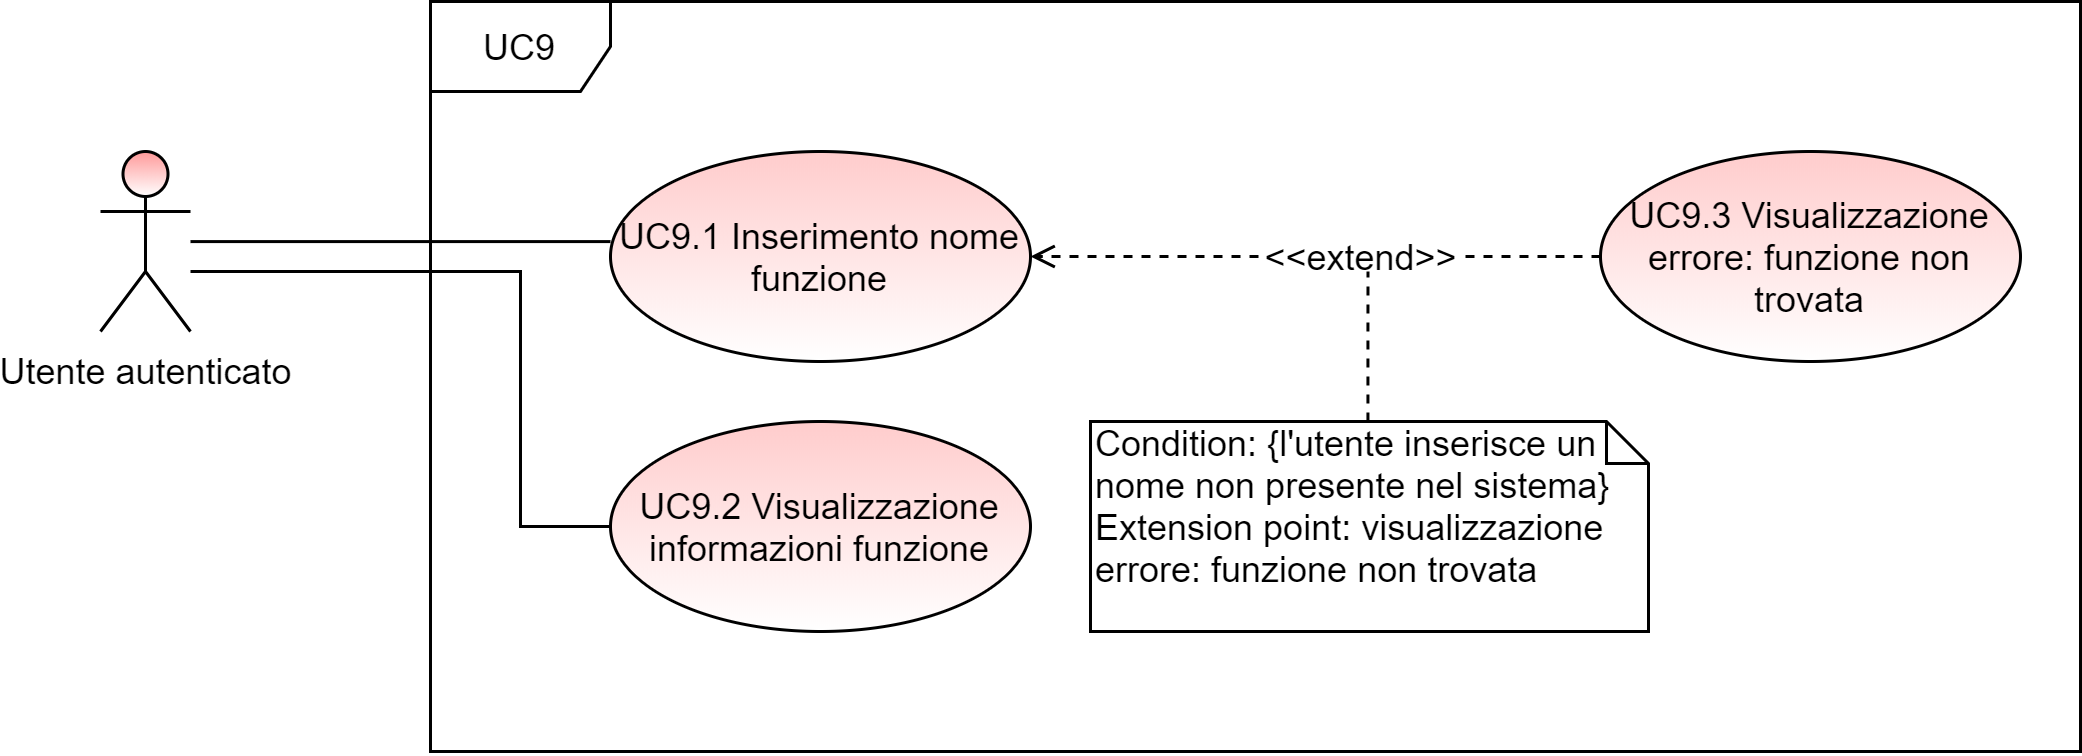
\includegraphics[scale=\ucs]{./res/img/UC9.png}
	\caption {UC9 - Ricerca funzione per nome}
\end{figure}
\begin{itemize}
	\item \textbf{Attori primari:} \ua{};
	\item \textbf{Attori secondari:} \re{};
	\item \textbf{Descrizione:} l’utente vuole visualizzazione una descrizione completa di una funzione di cui conosce il nome eseguendo il comando \pinfo{};	
	\item \textbf{Scenario principale:} l'utente richiede di visualizzare le informazioni dettagliate di una funzione tramite il comando \pinfo{};
	\item \textbf{Precondizione:} l'utente inserisce correttamente ed esegue il comando \pinfo{};
	\item \textbf{Postcondizione:} la ricerca della funzione tramite nome avviene correttamente. 
\end{itemize}